%%%%%%%%%%%%%%%%%%%%%%%%%%%%%%%%%%%%%%%%%
% Short Sectioned Assignment
% LaTeX Template
% Version 1.0 (5/5/12)
%
% This template has been downloaded from:
% http://www.LaTeXTemplates.com
%
% Original author:
% Frits Wenneker (http://www.howtotex.com)
%
% License:
% CC BY-NC-SA 3.0 (http://creativecommons.org/licenses/by-nc-sa/3.0/)
%
%%%%%%%%%%%%%%%%%%%%%%%%%%%%%%%%%%%%%%%%%

%----------------------------------------------------------------------------------------
%	PACKAGES AND OTHER DOCUMENT CONFIGURATIONS
%----------------------------------------------------------------------------------------

\documentclass[paper=a4, fontsize=11pt]{scrartcl} % A4 paper and 11pt font size

\usepackage[T1]{fontenc} % Use 8-bit encoding that has 256 glyphs
\usepackage{fourier} % Use the Adobe Utopia font for the document - comment this line to return to the LaTeX default
\usepackage[english]{babel} % English language/hyphenation
\usepackage{amsmath,amsfonts,amsthm} % Math packages
\usepackage{graphicx}            			% Figures
\usepackage{verbatim}            			% Code-Environment
\usepackage{url}
\usepackage{hyperref}					% links in pdf
\usepackage{cleveref}

\usepackage{lipsum} % Used for inserting dummy 'Lorem ipsum' text into the template

\usepackage{sectsty} % Allows customizing section commands
\allsectionsfont{\centering \normalfont\scshape} % Make all sections centered, the default font and small caps

\usepackage{fancyhdr} % Custom headers and footers
\pagestyle{fancyplain} % Makes all pages in the document conform to the custom headers and footers
\fancyhead{} % No page header - if you want one, create it in the same way as the footers below
\fancyfoot[L]{} % Empty left footer
\fancyfoot[C]{} % Empty center footer
\fancyfoot[R]{\thepage} % Page numbering for right footer
\renewcommand{\headrulewidth}{0pt} % Remove header underlines
\renewcommand{\footrulewidth}{0pt} % Remove footer underlines
\setlength{\headheight}{13.6pt} % Customize the height of the header

\numberwithin{equation}{section} % Number equations within sections (i.e. 1.1, 1.2, 2.1, 2.2 instead of 1, 2, 3, 4)
\numberwithin{figure}{section} % Number figures within sections (i.e. 1.1, 1.2, 2.1, 2.2 instead of 1, 2, 3, 4)
\numberwithin{table}{section} % Number tables within sections (i.e. 1.1, 1.2, 2.1, 2.2 instead of 1, 2, 3, 4)

\setlength\parindent{0pt} % Removes all indentation from paragraphs - comment this line for an assignment with lots of text

%----------------------------------------------------------------------------------------
%	TITLE SECTION
%----------------------------------------------------------------------------------------

\newcommand{\horrule}[1]{\rule{\linewidth}{#1}} % Create horizontal rule command with 1 argument of height

\title{	
\normalfont \normalsize 
\textsc{Technical university of Vienna} \\ [25pt] % Your university, school and/or department name(s)
\horrule{0.5pt} \\[0.4cm] % Thin top horizontal rule
\huge Master Thesis Contributions \\ % The assignment title
\horrule{2pt} \\[0.5cm] % Thick bottom horizontal rule
}

\author{Andreas Egger, 0626885} % Your name

\date{\normalsize\today} % Today's date or a custom date

\begin{document}

\maketitle % Print the title

%----------------------------------------------------------------------------------------
%	CONTRIBUTION TOPICS
%----------------------------------------------------------------------------------------

\section{Contribution Topics}

In the thesis different aspects are adressed from a range of different fields. The following constitutes an overview of the various topics and the motivation to include them in the thesis. 

%------------------------------------------------

\subsection{Simulation Scenario}

A simulation scenario is built to assess different metrics and characteristics of data centers in a distributed cloud environment. Different job lengths, server capacity and migration or delay constraints can be simulated within the environment. Various scenarios are set up to show potential cost savings when adding forecast or migration measures.  

%------------------------------------------------

\subsection{Forecasting}

Forecasting is important to compare future energy prices to estimate cost savings at some time range into the future, under the assumption of bandwidth constraints and/or SLAs (delay constraints) to avoid the excessive use of migrations. 

%------------------------------------------------

\subsection{Scheduling}

A custom scheduler is set up that can handle several scenarios and define conditions when VMs should be migrated to other locations to save energy costs. 
Depending on the scenario resources may be allocated to different locations depending on the type of SLA or migration constraints that are valid for the scenario. 

%------------------------------------------------

\subsection{Electricity price data}

The simulation is based on real electricity price data from various energy markets in Europe and the USA. Under the assumption that each data center is taking part in an energy exchange with an energy market actual cost savings can be deduced from the simulation scenario. 

%------------------------------------------------

\subsection{Reusable architecture for cloud environment}

A framework has been built to collect and save energy price data, analyse and create forecasting models based on given data and provide generic interfaces that can be accessed by other components or frameworks where forecasts and price data can be retrieved dynamically. 

%------------------------------------------------


%----------------------------------------------------------------------------------------
%	OUTLINE
%----------------------------------------------------------------------------------------

\section{Outline}

%------------------------------------------------

\subsection{Forecasting}

To illustrate the benefit of forecasting in a cloud environment the forecast comparison of two price time series is depicted in figure \ref{fig:Da_Prices_Forecast}. 

Depending on the length of the running job price forecasts would be calculated to encompass the whole time range of the job. When comparing different forecasted price curves it can be estimated if and when it is best to migrate jobs to another data center. Taking into account constraints such as migration costs or SLA penalties it is not beneficial to migrate jobs too often, e.g.~at each timestamp. Thus it is important to make sure that migrations happen infrequently but with a high probability of saving costs, taking into account some level of uncertainty from forecasts. 

%------------------------------------------------

\subsection{Block diagram}

The block diagram in figure \ref{fig:Block_Diagram_Architecture} shows all components and interfaces existing in the implementation. It provides a good overview of the interaction between components and their role within the architecture. 

The import module imports energy price data from different energy markets which is transformed and saved into a database. The scheduler periodically checks for new data and triggers the import as well as the forecast model generation for the newly retrieved data. 

The forecast generation is done on a separate R Server which is then stored and provided to the application server. Data and forecast interfaces are established which can be used by other applications such as the Cloud Simulator. It is possible that these interfaces are used by a real cloud as well since they can be made publicly available. 

%------------------------------------------------

\subsection{Component Diagram}

The component diagram shows the architecture in more detail and reveals some implementation level interfaces (figure \ref{fig:Component_Diagram}). It shows relationships between the cloud environment, the forecasting components and the application server. 

The cloud framework component represents the simulation environment including the scheduler and simulator. The simulator is responsible for generating job requests and setting up the cloud environment to be used by the scheduler. 

The scheduler takes current job and migration requests and determines the right strategy based on the selected simulation scenario. SLA and capacity constraints can be taken into account as well as forecasted energy prices. 

The data is retrieved from the data processing and forecasting component which is responsible for data fetch and forecast calculation. The data interface component is responsible for fetching and parsing the data and saving it to the database. 

Energy price data is fetched from the database by the forecasting component which generates forecast models based on the data. During the process the best model is selected and forecasted prices are served to other components via the forecast interface. 

\hspace{4cm}

\begin{figure}[htbp]
	\centering
		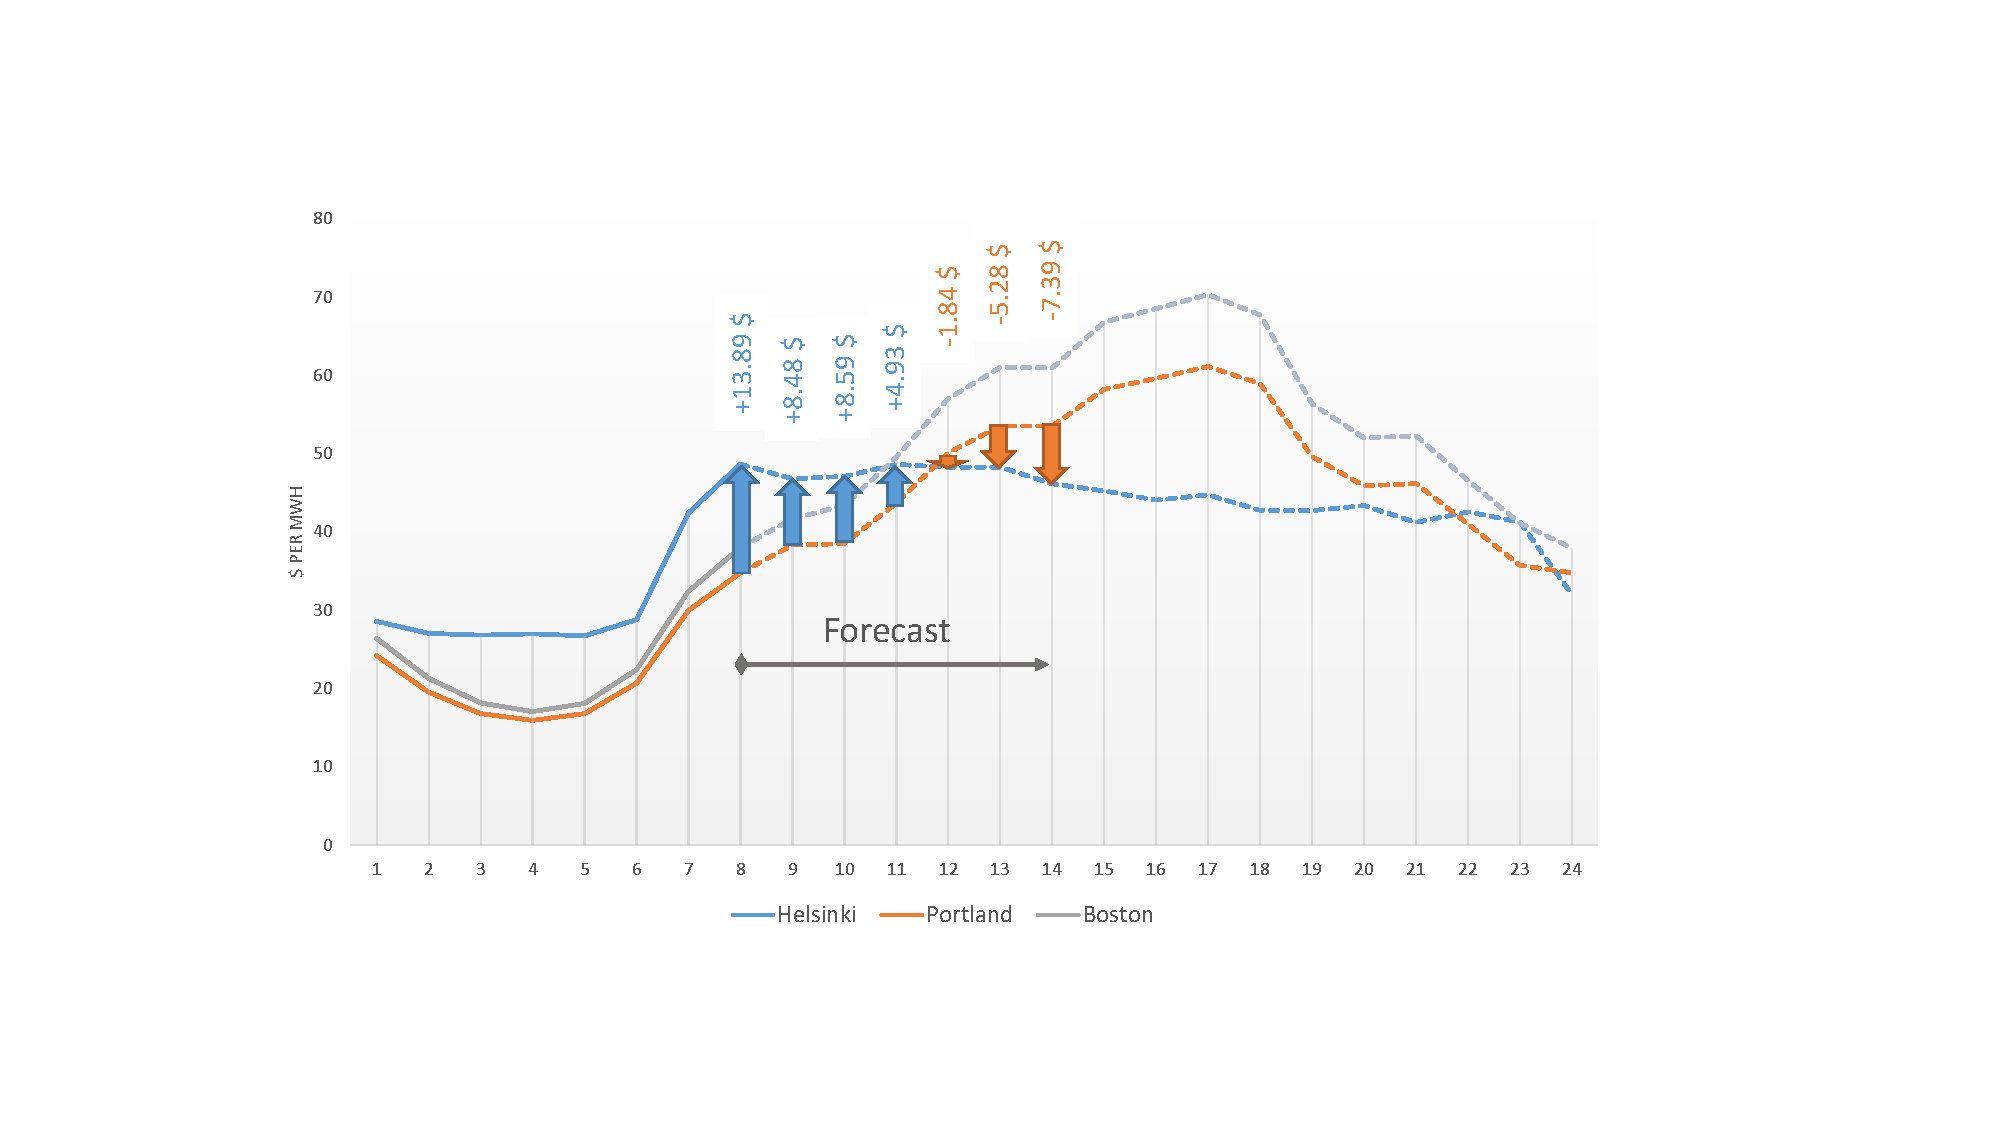
\includegraphics[width=\textwidth]{figures/Da_Prices_Forecast_Illustrated.png}
	\caption{Illustration of day ahead price comparison in forecasting}
	\label{fig:Da_Prices_Forecast}
\end{figure}

\begin{figure}[htbp]
	\centering
		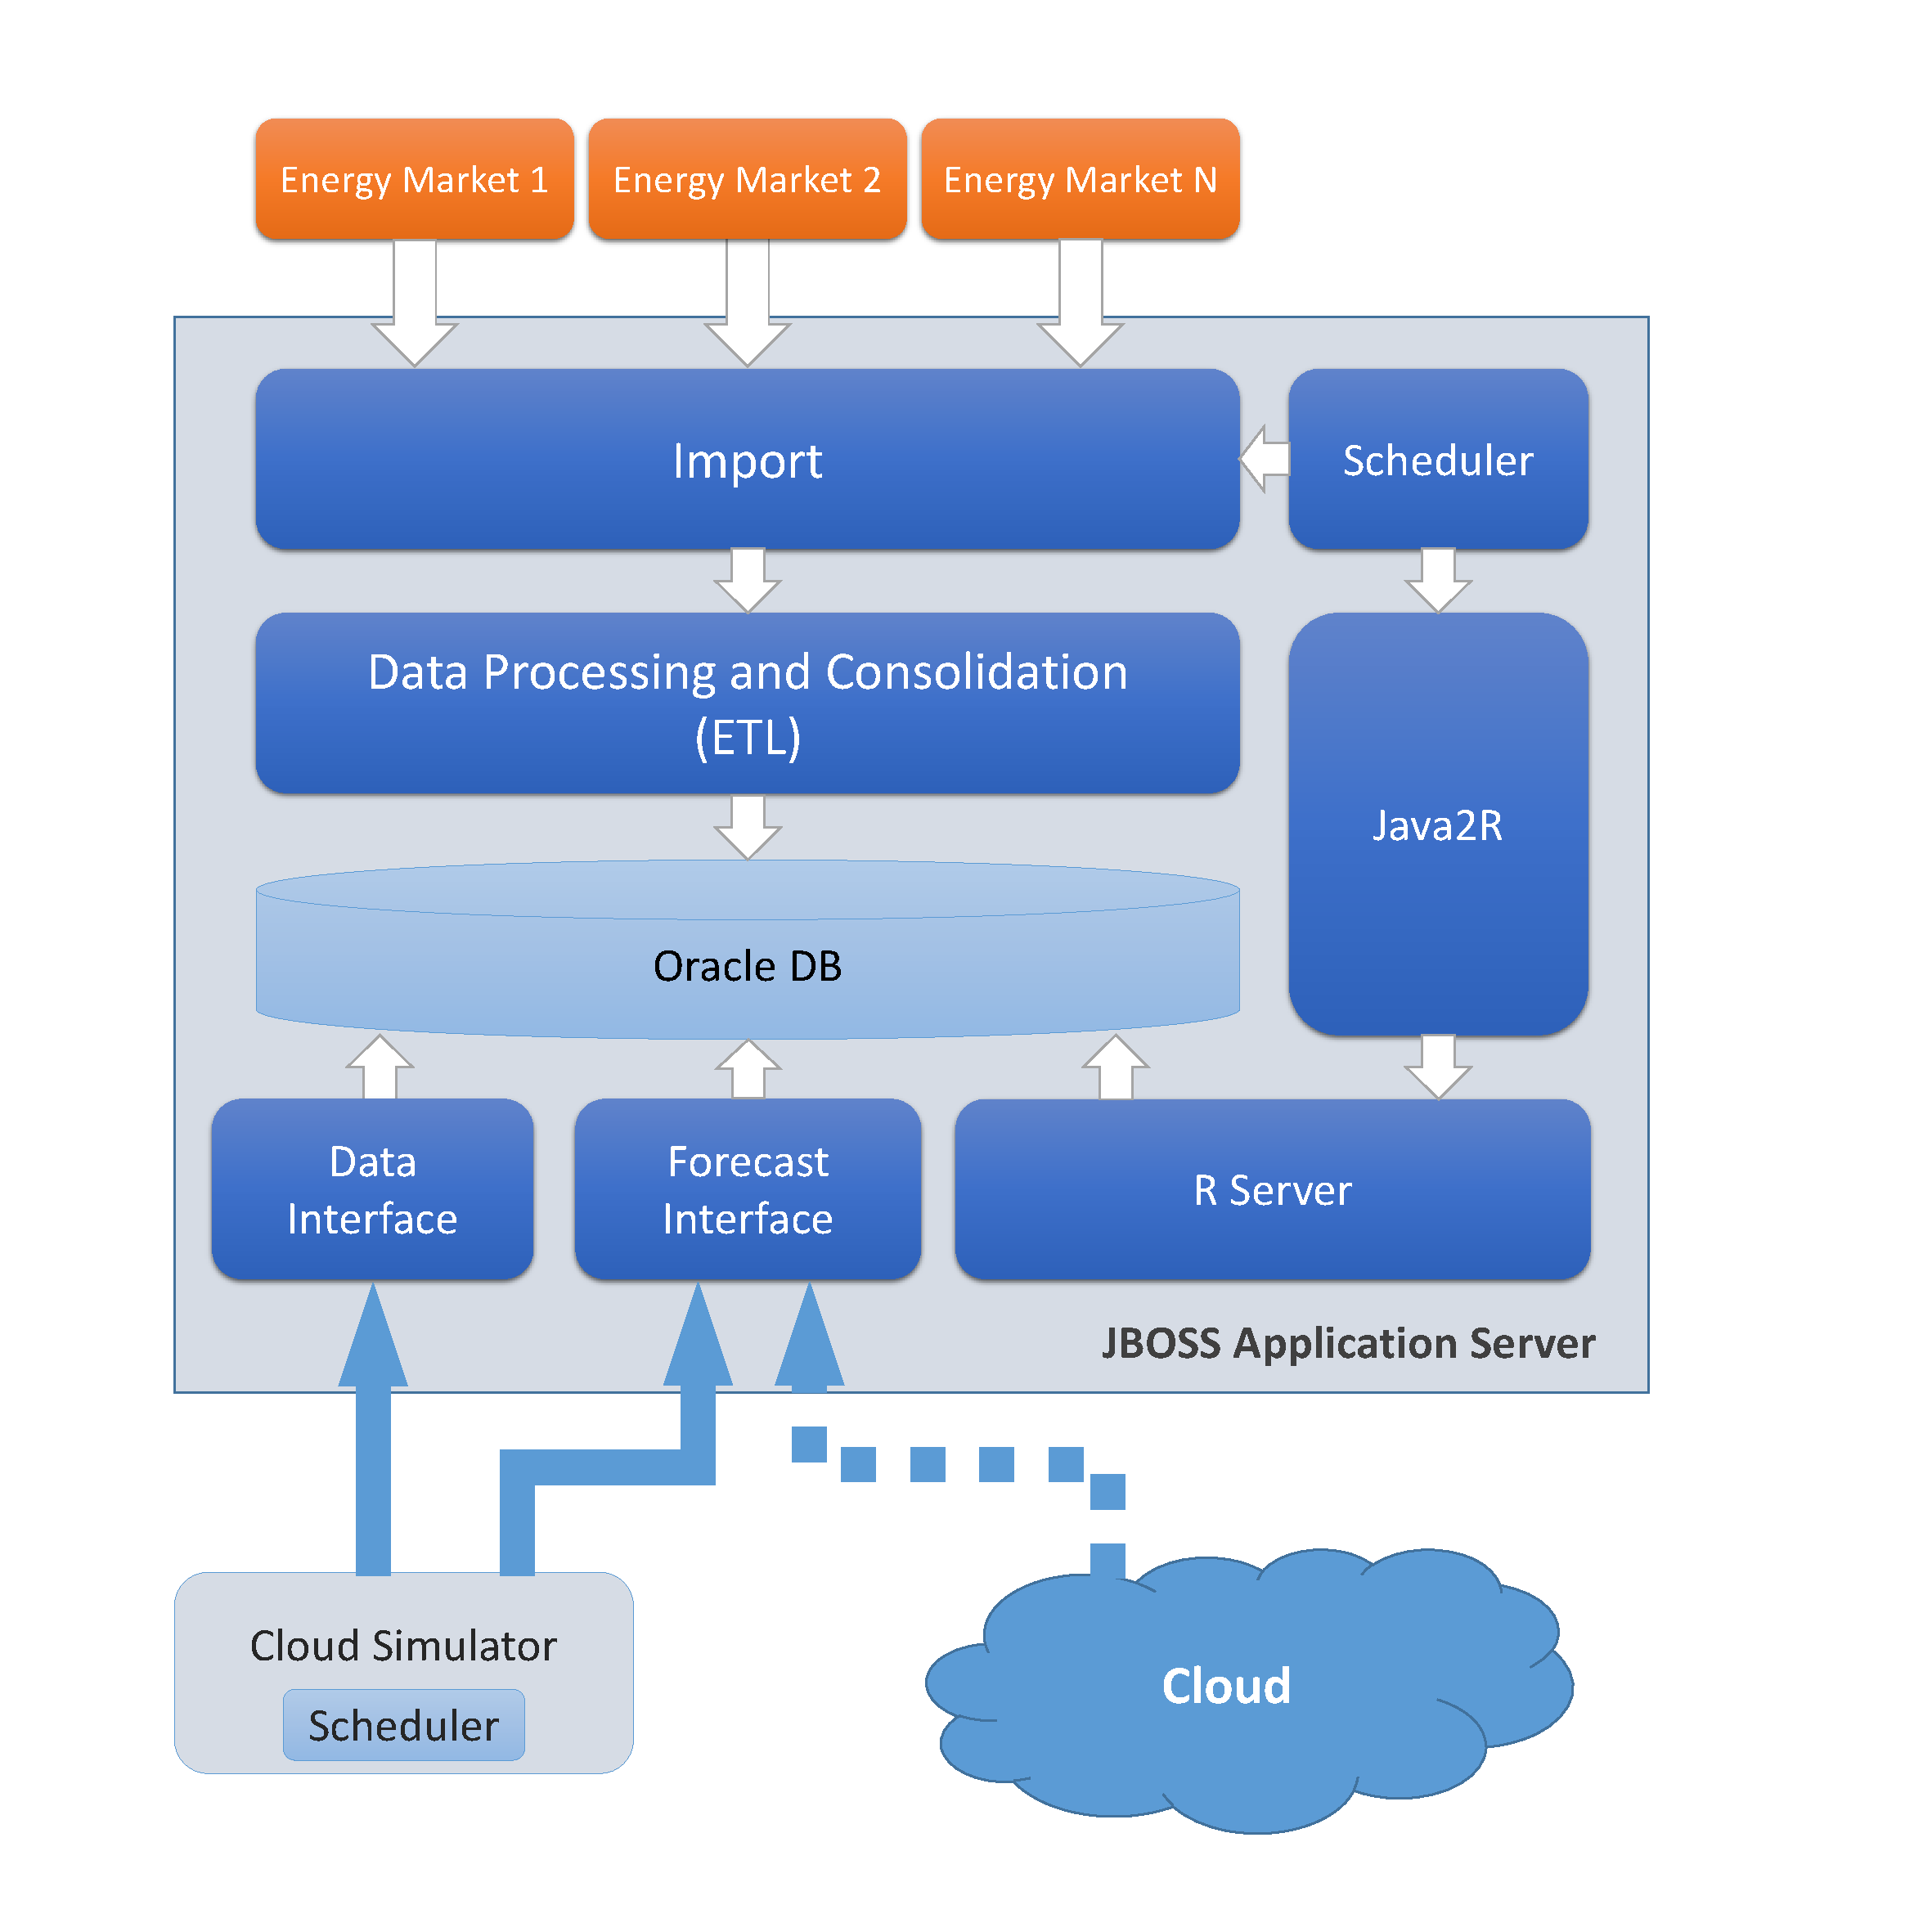
\includegraphics[width=0.9\textwidth]{figures/Block_Diagram_Architecture.pdf}
	\caption{Architecture Block Diagram}
	\label{fig:Block_Diagram_Architecture}
\end{figure}

\begin{figure}[htbp]
	% used to position the image at the horizontal center of the page
	\hspace*{-0.4in}
		% include the graphic rotated by a 90 degree angle and scale to paperwidth and height
		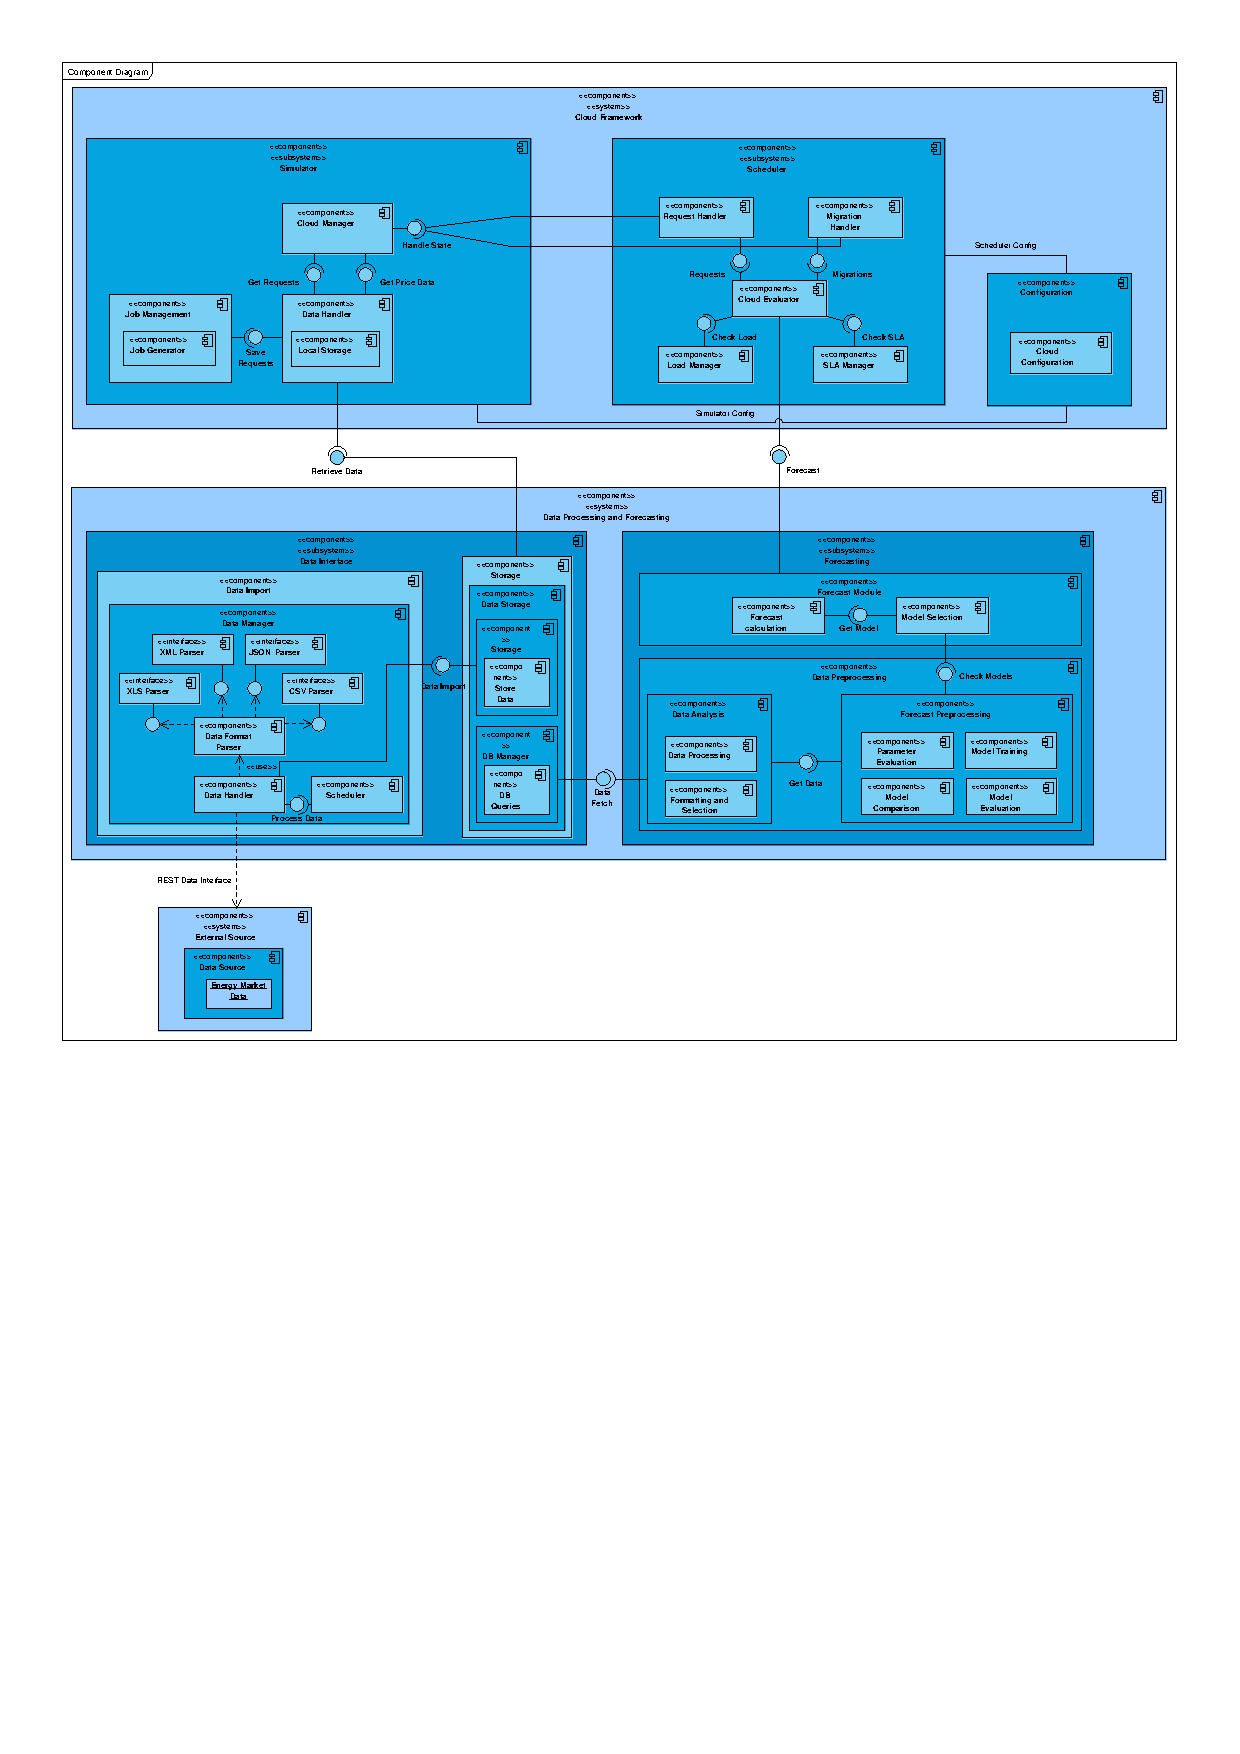
\includegraphics[angle=90,width=\paperheight,height=\paperwidth,keepaspectratio=true]{figures/Component_Diagram.pdf}
	\caption{Component Diagram}
	\label{fig:Component_Diagram}
\end{figure}


\newpage

%----------------------------------------------------------------------------------------
%	IMPLEMENTATION
%----------------------------------------------------------------------------------------

\section{Implementation}

The practical part of the thesis consists of three components which interact with each other to provide the desired results. 

%------------------------------------------------

\subsection{Application Server}

Automatic fetch of electricity spot prices from various energy market sources, parsing and transforming data into a common format and saving prices to a database for later retrieval. Parsers for retrieving and transforming energy prices from various energy markets have been implemented whereas the architecture has been kept modular to allow to easily add new parsers and resources. 

%------------------------------------------------

\subsection{R Forecasting}

Implement model training and evaluation in R, investigate time series and forecast accuracy to build suitable models for a specific data set. Models are trained for a given data set to provide effective and optimal forecasts for the given data. Functions have been implemented to analyse the data set and compare generated models to choose the model with the best accuracy. 

%------------------------------------------------

\subsection{Python Simulator (partly contributed)}

The python simulator is responsible for creating the cloud and modeling of constraints that shape the outcome of the simulation. It is capable of running simulations of various scenarios and configurations, archive inputs and output results in python plots and charts. As part of the contribution to this thesis an own scheduler and configuration file has been set up and access to web services has been implemented. New data and plots and an archive function have been implemented as well.


%----------------------------------------------------------------------------------------
%	INTERFACES
%----------------------------------------------------------------------------------------

\section{Interfaces}

%------------------------------------------------

\subsection{Application Server}

The application server provides web service interfaces to retrieve the previously stored energy prices and results of forecasting calculations. It accesses R methods on a natively running R Server and triggers functions to generate forecasting models and executes and saves the output of the models in its internal state. The results of the forecasting calculations as well as the stored energy prices can be queried via the web service interfaces (e.g. by the simulator). 

%------------------------------------------------

\subsection{R Server}

The R Server is running on the local machine to provide access to functions for generating and evaluating forecasting models and retrieving the results. This is advantegous since computationally expensive operations can be outsourced and used by other applications (e.g. the application server). 

%------------------------------------------------

\subsection{Simulator}

The simulator provides configuration files to easily amend the output of a simulation by overriding values that are used within the simulation. It is able to make calls to web service interfaces (e.g. from the application server) to query energy prices and forecasting results. 


%----------------------------------------------------------------------------------------

\end{document}